\chapter{Firewall and Network Security}

Protecting information can be more complex than protecting phyisical goods.
We may be interested in preventing that information can be duplicated or read by third parties.
We may want to also protect information from being modified or erased.

The internet makes it possible for the information to easily travel accross the globe.
All the protocols and tools that are typically used with good intentions can also be used to abuse and exploit information systems.
Therefore, it is important to keep security in mind when designing and managing information networks.

Security can be present at different layers of the protocol stack.
For example, the TLS protocol offers security at the application layer in the internet protocol stack.
TLS is used to protect HTTP sessions in the HTTPS protocol. 
The open source implementation of TSL OpenSSL was recently in the news after the heartbleed bug was discovered.

IPsec offers security at the network layer.
It can be used to protect all traffic between two endpoints.
These endpoints can be either a host or a network.
IPsec uses two different forms of protection.
The Authentication Header (AH) provides integrity, data origin authentication and protection against replay attacks.
The Encapsulating Security Payload (ESP) header provides confidentiality, data origin authentication, integrity and protection against replay attacks.

IPsec can operate in two different modes: transport mode and tunnel mode.
In the first one, the payload of an IP packet is protected while the IP headers are left unmodified.
In the second mode of operation, IPsec tunnel mode, the entire IP packet is protected and encapsulated within a new IP packet.

Another aspect of security is access control and network perimeter protection.
It is desired to prevent unauthorized access to computers and networking devices.
In the internet there are automatized tools that are continuously looking for vulnerabilities to gain unauthorized access to systems.
Botnets are hordes of infected computers (also called zombies) that follow the commands of a master and can be used to send spam, perform port scans, or search for vulnerable systems.

Keeping the software updated and using strong passwords helps in keeping systems secure.
Another tool that helps in protecting networks and computers are firewalls.
Firewalls filter traffic and stop undesired and potentially malicious packets.
The firewall can be installed in an end computer, to protect only that computer, or in a networking device to protect a network.
We will be focusing on the latter kind of firewall.

\section{Firewall}

A network can be protected from attacks coming from the rest of the internet by placing a firewall in the frontier between the two networks.
To be effective, it is important that all the traffic exchanged by the network and the rest of the internet goes through the firewall.
The firewall filters undesired traffic to offer partial protection against external attacks.
Note that a negative aspect of forcing that all the traffic between our network and the internet is handled by the firewall is that it introduces a single point of failure.
It is possible to have two firewalls with the same configuration to mitigate this problem.

In perimeter protection, networks are called security domains and are classified regarding their level of trust.
For example, the network of the organization can be considered trusted and therefore it is a trusted security domain.
The public internet can be considered untrusted and it is therefore an unstrusted security domain.
A firewall is placed between the two of them to enforce access control rules.
The firewall protects the trusted domain from the unstrusted domain.

More complex topologies are possible.
For example it is possible to have multiple nested security domains with multiple firewalls securing each of them.
In this case, the network that is considered trusted by one firewall is considered untrusted by another firewall.
This situation is illustrated in Fig.~\ref{fig:Nested_security_domains}.

\begin{figure}
\centering
\ifpdf
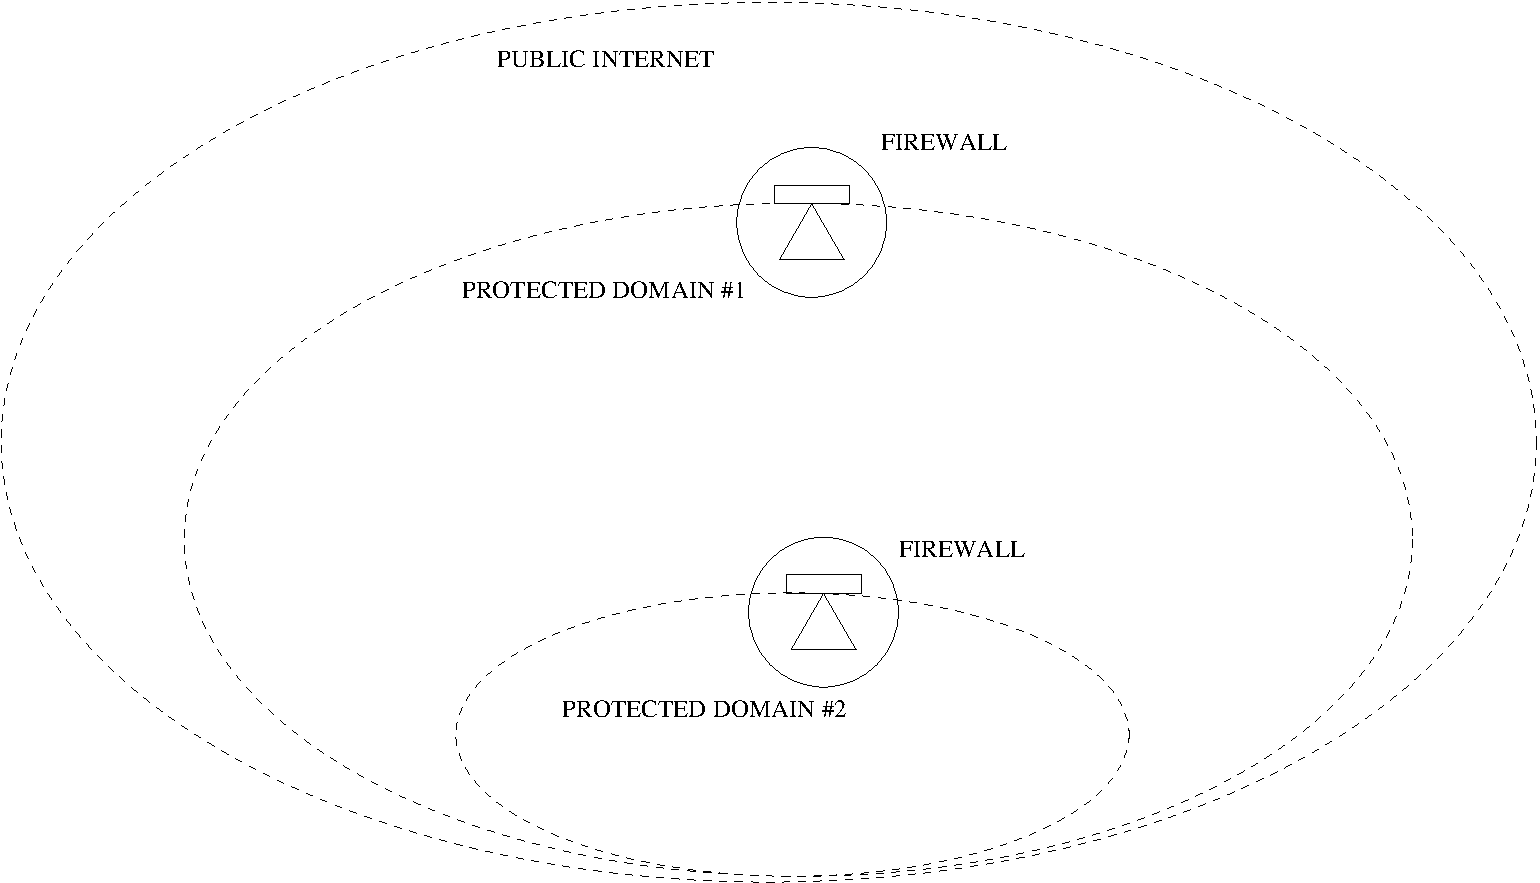
\includegraphics[width=0.5\linewidth]{Figures/Nested_security_domains.pdf}
\else
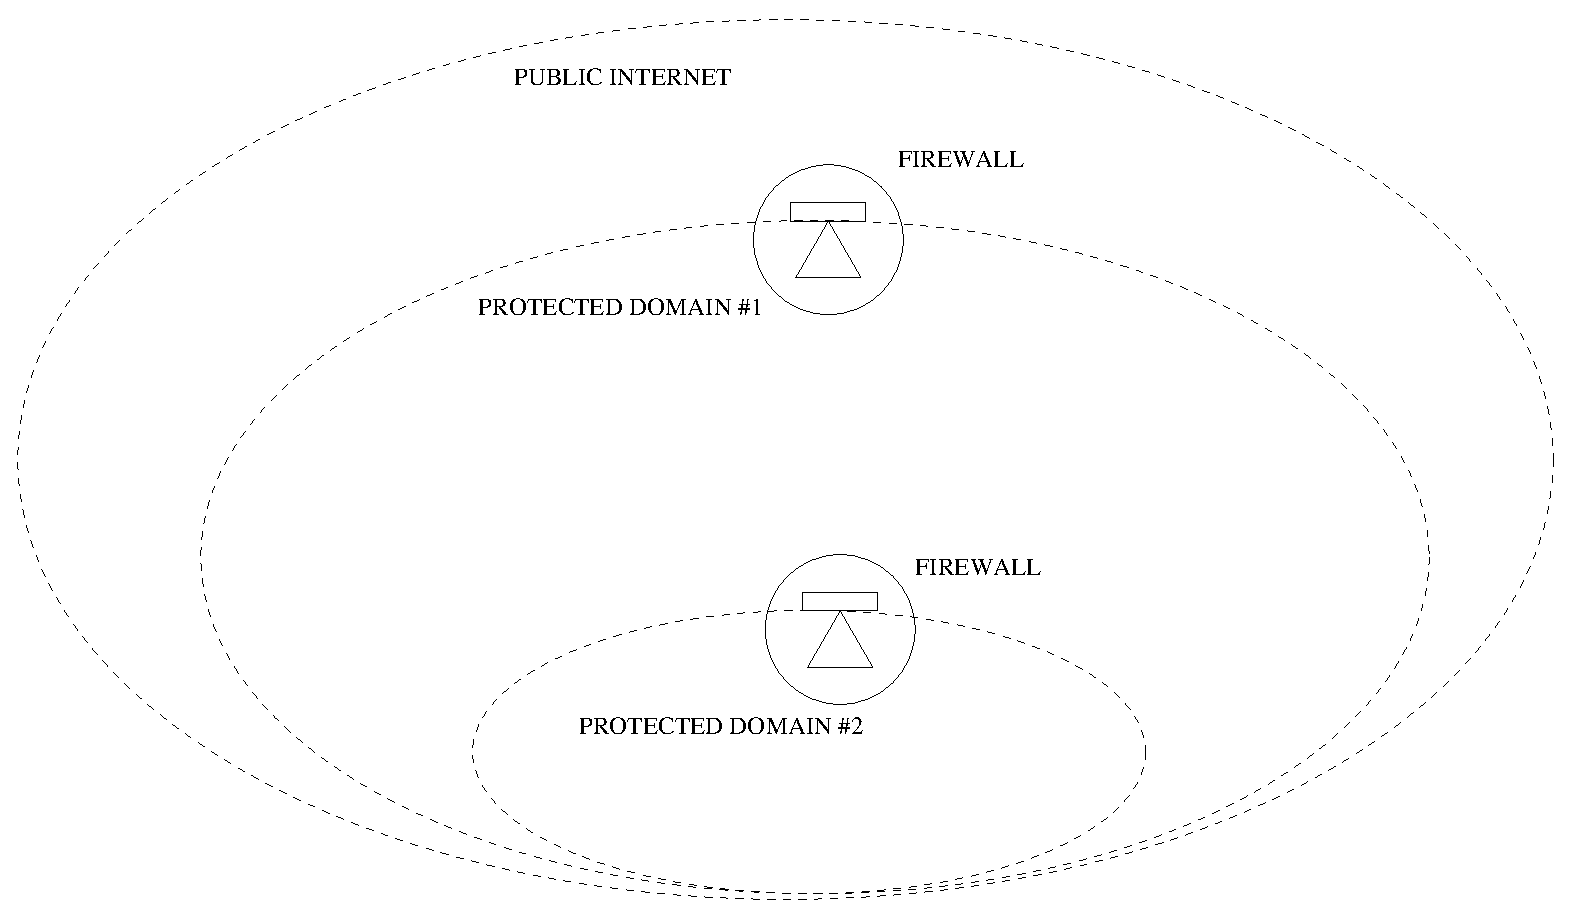
\includegraphics[width=0.5\linewidth]{Figures/Nested_security_domains.eps}
\fi
\caption{Nested security domains.}
\label{fig:Nested_security_domains}
\end{figure}

Another common situation is that an organization wants to expose some information to the internet, for example using web servers.
This web servers need to be placed in a network that can be accessed from the outside.
It is still possible to offer partial protection to this servers using a firewall.
For example, the firewall can be configured to allow only web traffic between the internet and the network of the web servers.
This partially protected network is typically named DMZ (for demilitarized zone).
The organization can keep a network totally protected (internal) and another network partially protected (DMZ), as shown in Fig.~\ref{fig:DMZ}.

\begin{figure}
\centering
\ifpdf
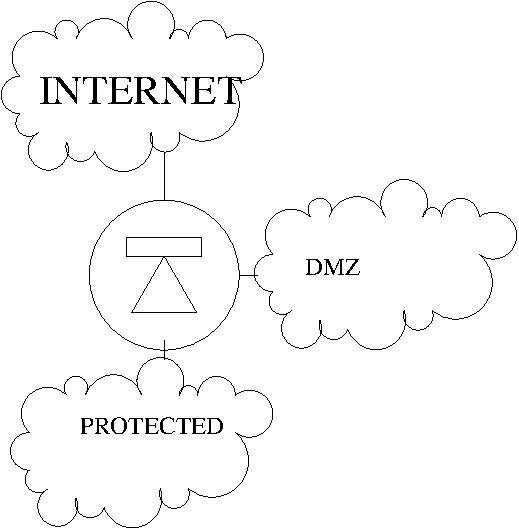
\includegraphics[width=0.5\linewidth]{Figures/DMZ.pdf}
\else
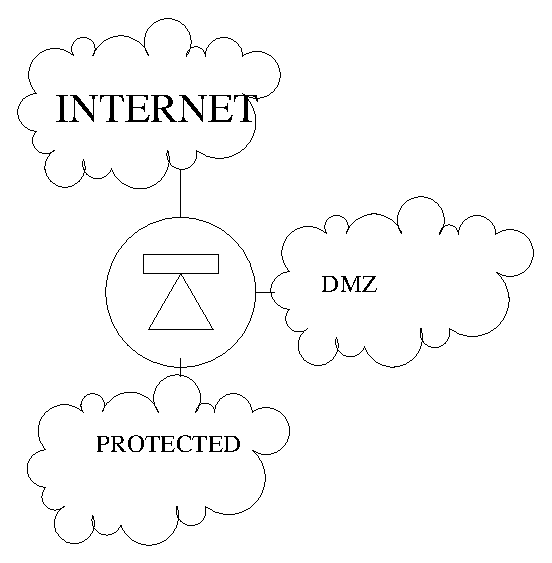
\includegraphics[width=0.5\linewidth]{Figures/DMZ.eps}
\fi
\caption{The firewall separates the public internet, the protected network and a DMZ.}
\label{fig:DMZ}
\end{figure}

There are two possible options to separate the trusted and untrusted domains.
The first one is physical separation, in which the two domains use different hardware.
The second option is logical separation, in which the two domains share some hardware and are logically separated using VLANs or MPLS tags.
Physical separation is considered safer than logical separation.

\subsection{Chain of rules}

There are also to different approaches when configuring a firewall: Permissive access control (reactive) and restrictive access control (proactive).
In the first one, traffic is allowed unless explicitly forbidden.
If a threat is detected, the network administrator adds a new rule to the firewall to protect the network from the threat.
In restrictive access control, the traffic is forbidden unless explicitly allowed.
When a new service requires to send packets through the firewall, the network administrator adds new rules to the firewall to permit the traffic associated to the new service.

A firewall is typically implemented as a chain of rules that are checked one by one until one of the rules matches.
When there is match, the rule has an associated action that can be either allow or deny.
In the case of a restrictive firewall the last rule of the chain denies (rejects) all traffic that does not match any of the previous rules.
In a permissive firewall, the last rules allows any traffic that has not been dropped by any of the previous rules.

The following listing shows an example of a restrictive set of rules:
\begin{lstlisting}
Src             Dst     Protocol        Service            Action
192.168.1.11/32 any     tcp             80                  Allow
192.168.1.0/24  any     any             any                 Drop
any             any     udp             53                  Allow
any             any     any             any                 Drop
\end{lstlisting}

The rules chain applies to a particular interface and a particular direction of traffic.

\subsection{Stateless Firewall}

In its simplest form, a firewall takes decisions based uniquely on the headers of the packet.
This information can include information regarding IP addresses, layer 4 protocol and ports.
For example, a firewall allowing only packets to and from a particular host could be implemented as a stateless firewall.
A firewall that allows all packets that use port 80 as a source or destination port could also be implemented with a stateless firewall.

\subsection{Stateful Firewall}

Consider the previous example of allowing all packets that contain port 80 as either its source or destination port.
This configuration allows the computer in the protected network to browse the web available in servers of the public internet.
A problem with this configuration is that any host of the public internet can access any computer and any port in the protected network by simply using port 80 as its source port.
This configuration gives little protection to the protected network.

An alternative to allow the computers in the protected network to visit web browsers in the public internet while keeping the protected network more secure is to use a stateful firewall.
The stateful firewalls keeps the state of a connection and can take a decision about whether to allow or reject a packet taking into account the history of packets that have traversed the network before.
When a client in the protected network sends a packet to a web server in the public internet, the firewall stores the addresses and ports of this packet in a database and then will allow the packets that are answering this particular request.
Compared to the stateless firewall that accepted all packets that used port 80, the stateful firewall accepts only those packets that are answering a request initiated in the protected network.
Stateful firewalls are much more effective and therefore are the firewalls that we normally use nowadays.

\section{Related Security Concepts}

\subsection{Deep Packet Inspection}

Normal firewalls consider only information available in the network layer and the transport layer of the packet.
Deep packet inspection (DPI) is about re-constructing application layer messages and taking decisions based on this information.
A deep packet inspection firewall can differentiate between a web packet and file sharing packet even if they both use exactly the same IP and port information.
A DPI can be much more precise in making decisions thanks to the additional information it has access to.

The problem is that the number of applications is very large and is growing continuously.
It is difficult to keep track of all existing applications. 
Furthermore, looking into the application messages and interpreting application information is computationally expensive and consumes CPU time.
Therefore, the packet processing speed is much lower for DPI than it is for normal firewall operation.
Some applications encrypt the information making it more difficult or impossible for the DPI firewall to extract information from the application layer.

\subsection{Intrusion Detection and Prevention Systems}

An intrusion detection system (IDS) is a device or software that continuously monitors network traffic to detect anomalies that can be indicative of an attack.
We can differentiate to kinds of IDS:
\begin{itemize}
\item Signature-based: The IDS has a database of signatures of virus and malicious packets in general.
The IDS continuously compares the network packets with the signature database and rises an alarm when malicious packets are detected.
It is important to keep updating the database as new attacks are discovered.
\item Statistics-based: The IDS gathers statistics about \emph{normal} traffic behaviour.
Then, it continuously compares traffic statistics with what is considered normal and rises an alarm when it detects abnormal traffic patterns.
\end{itemize}

IDS have the problem of issuing false positives and false negatives.
In a false positive event, an alarm is raised when there is no attack situation.
In a false negative event, an attack goes undetected.

An intrusion prevention system (IPS) is an IDS that has the capability to automatically take action to prevent the attack.
An IPS can, for example, change the firewall rules to stop malicious traffic.

\subsection{Application Layer Gateway}

An Application Layer Gateway (ALG) works in combination with a firewall to interpret messages at the application layer as in DPI.
An ALG uses the information to adjust the firewall rules or to rewrite the message to allow legitimate user communication through the firewall.
The ALG is intended for protocols that open additional ports to perform their task, such as SIP, FTP and BitTorrent.

\section{Network Address Translation and Port Address Translation}

Network address translation (NAT) translates addresses between two domains.
When the protected domain uses private addresses, NAT is required to translate those addresses to public internet addresses.

\subsection{Static mapping NAT}
In its simplest form, NAT is a one-to-one mapping.
For example, private address 192.198.1.1 could be translated to a public address 193.145.56.1.
This translation can be bi-directional, and all packets arriving at the public-facing interface can be translated to the corresponding private address.
With this kind of mapping, a client in the public internet can contact a server in the private IP addressing space if it knows the corresponding public address.

\subsection{Dynamic mapping NAT}
In a more complex situation, several devices on the private address space share a set of public addresses.
In this situation, the NAT device dynamically uses public addresses for translating the private addresses.
The NAT device can take advantage of statistical multiplexing.
If the devices with private address are not always online, it is possible to use a set of public address to serve a larger number of devices.
The same device will probably be mapped to different public IP addresses at different times.
As this is no longer a one-to-one correspondence, it can be more complicated to host a server using the private address space its public equivalent address it is not always the same.


Despite the fact that in general there is not a one-to-one mapping between private and public addresses, if we look at any particular time instant there is a one-to-one mapping between those private addresses that are active and the public addresses.
The difference with static NAT is that in static NAT this one-to-one correspondence is valid for any period of time, while in dynamic NAT the one-to-one correspondence is valid only for a particular instant and can change dynamically.
The devices in the private address space take turns in using the public addresses, but they do not use them simultaneously.

The number of devices with private addresses that can simultaneously access the public internet is limited by the size of the pool of available public addresses.

\subsection{Port Address Translation}

Port address translation (PAT) allows that different devices with private addresses simultaneously use the same public address.
In NAT/PAT, both IP addresses and port numbers are translated.
The NAT/PAT device keeps a database with the association of address and port in the public side and the private side.
Each entry in the database has four fields: original address, original port, translated address and translated port.
Two different private addresses can be translated to the same public address as long as the resultant translation has different ports and therefore the translated address and translated port tuple is unique.

If two devices in the private network send a web request to the same webserver, the two packets will have different source addresses in the private network.
When this packets are translated by the NAT/PAT device, they will have the same source and destination address, but they will have different source ports.
The two reply answers from the webserver will have the same source and destination ports and different port destination number.
When receiving the two answers, the NAT/PAT device will differentiate the two packets using the different destination ports.
In the database in the NAT/PAT device there will be stored the private addresses that had originally initiated the web requests.
The NAT/PAT device will translate the two packets coming from the webserver using the two different addresses in the database and send the reply packets to the two devices that had originated the request.

PAT is also known as masquerading.

In principle, it is not possible for a client in the public internet to access a server in the private network unless port forwarding is used.

\subsection{Port Forwarding}

PAT is very useful when the number of public addresses available is limited and also to hide internal network topology.
Still, there are occasions in which is desirable to host a server in the private network behind the NAT/PAT.
If it is not possible assign a public address to the server in the NAT/PAT device, an option is to assign it an address and port tuple.
When the NAT/PAT device receives a packet in the public-facing interface that is directed to specified address and port tuple, it applies a static translation rule and directs it to the server behind the NAT/PAT.

For example, in a private network with a SMTP server and a web server installed in different hosts and with different private addresses, it is possible to install static rules in the NAT/PAT device that redirects some traffic arriving to the NAT/PAT public interface to the appropriate server.
In particular, there will be a rule that redirects traffic with destination port 80 to the webserver and with destination port 25 to the email server.
